
\chapter*{}
\addcontentsline{toc}{chapter}{\textsl{Diwar Les Coet}}

\section*{\textsl{Diwar Les Coet}}

\label{dlcscore}

\begin{center} 
\textbf{Composition Ouverte Opus 1}

{\scriptsize  \texttt{Copyleft \textcopyleft \, 2014/2017 Yann Ics - All Wrongs Reserved.}}
 \end{center} 
 \begin{figure}[H]
%\begin{center}
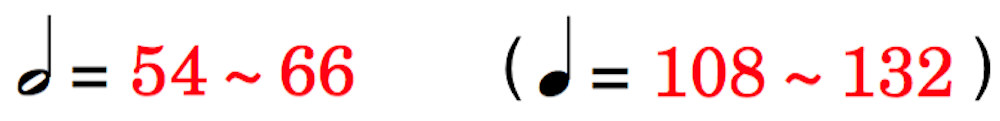
\includegraphics[scale=0.1]{img/dlct}
%\end{center}
\end{figure}
 
 Le tempo est purement indicatif et peut varier significativement et de mani\`{e}re dynamique, pourvu qu'il soit partager par tous les acteurs de la performance, qu'il soit synchronis\'{e} ou non.

\subsection*{Choral}

Initialement \'{e}crit pour 3 voix d'hommes, le choral peut \^{e}tre interpr\'{e}t\'{e} librement par toutes les voix et adapt\'{e} par octaviation. Les notes longues peuvent \^{e}tre monnay\'{e}es ou vocalis\'{e}es \`{a} loisirs selon le (con)texte. 

 \begin{figure}[H]
\begin{center}
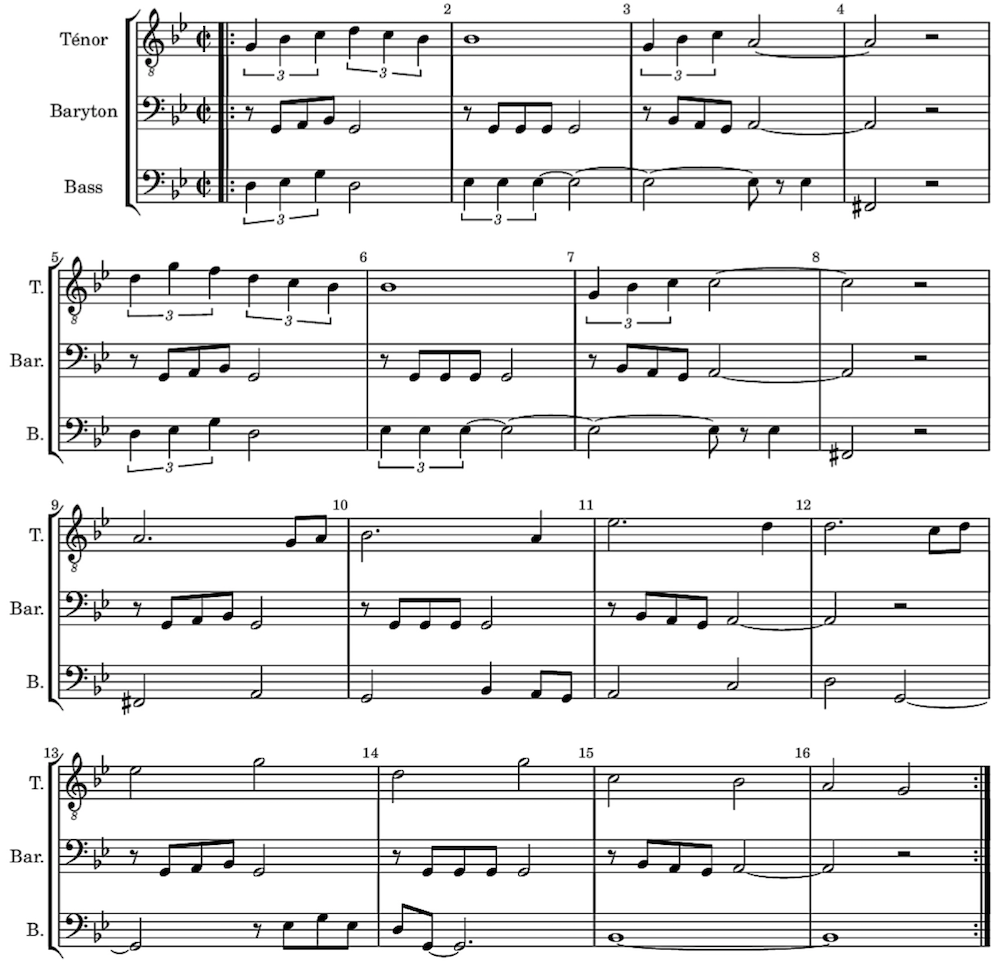
\includegraphics[scale=0.68]{img/dlc1}
\end{center}
\end{figure}

Pour certain passage, une version murmur\'{e}e ou bouche ferm\'{e}e entre bien entendu dans le domaine du possible.

%Le choral peut faire office de choeur et \^{e}tre accompagn\'{e} d'une (ou de) m\'{e}lodie(s) soliste(s).

Voici les combinaisons possibles (1 =  t\'{e}nor, 2 = baryton et 3 =  bass): 

1-- 2 -- 3 -- 12 -- 13 -- 23 -- 123

\subsection*{Variations pour Guitares}
Les grilles d'accords des guitares sont indicatives et peuvent par cons\'{e}quent \^{e}tre adapt\'{e}es librement au jeu du guitariste ou modifi\'{e}es selon l'interpr\'{e}tation souhait\'{e}e. La premi\`{e}re grille \'{e}tant la r\'{e}f\'{e}rence harmonique simplifi\'{e}e.

 \begin{figure}[H]
\begin{center}
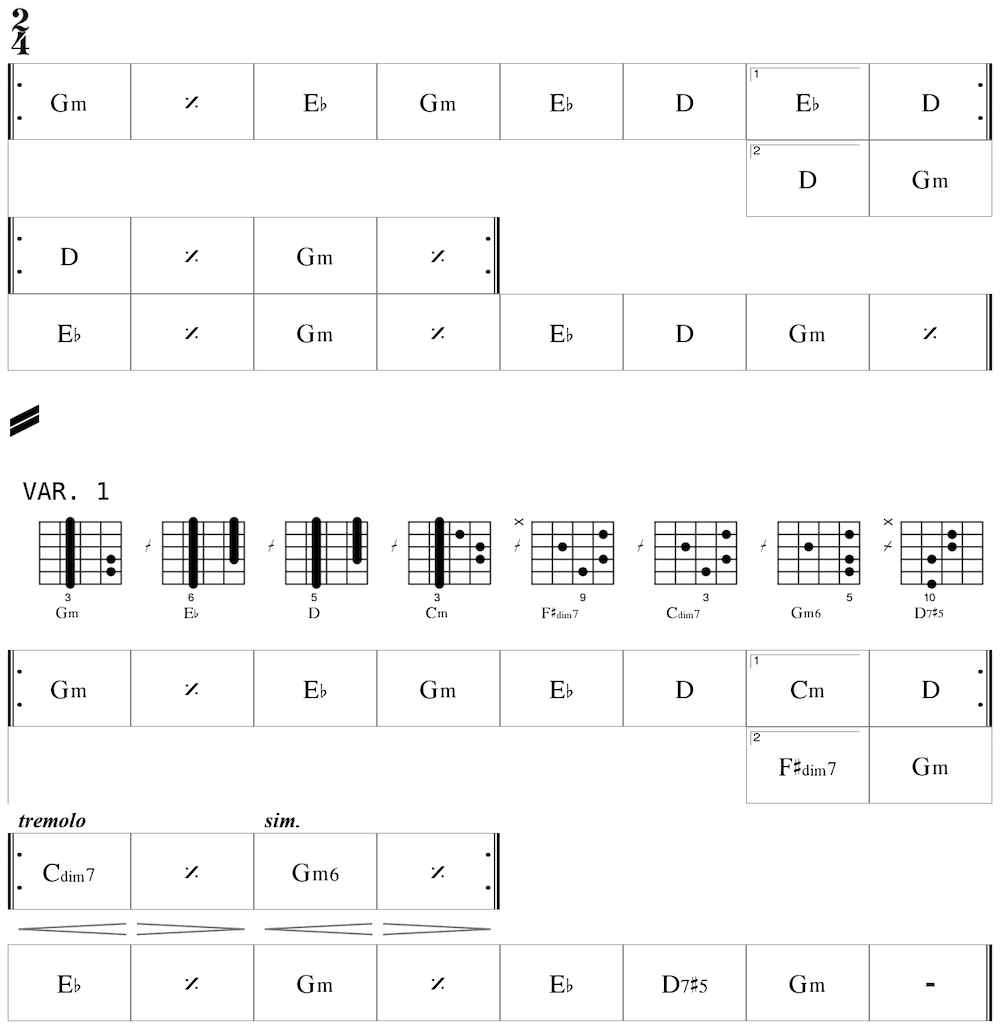
\includegraphics[width=\textwidth]{img/dlc2}
\end{center}
\end{figure}
Le cas \'{e}ch\'{e}ant, les grilles harmoniques peuvent \^{e}tre r\'{e}alis\'{e}es par n'importe quel instrument ou formation.
 
 \begin{figure}[H]
\begin{center}
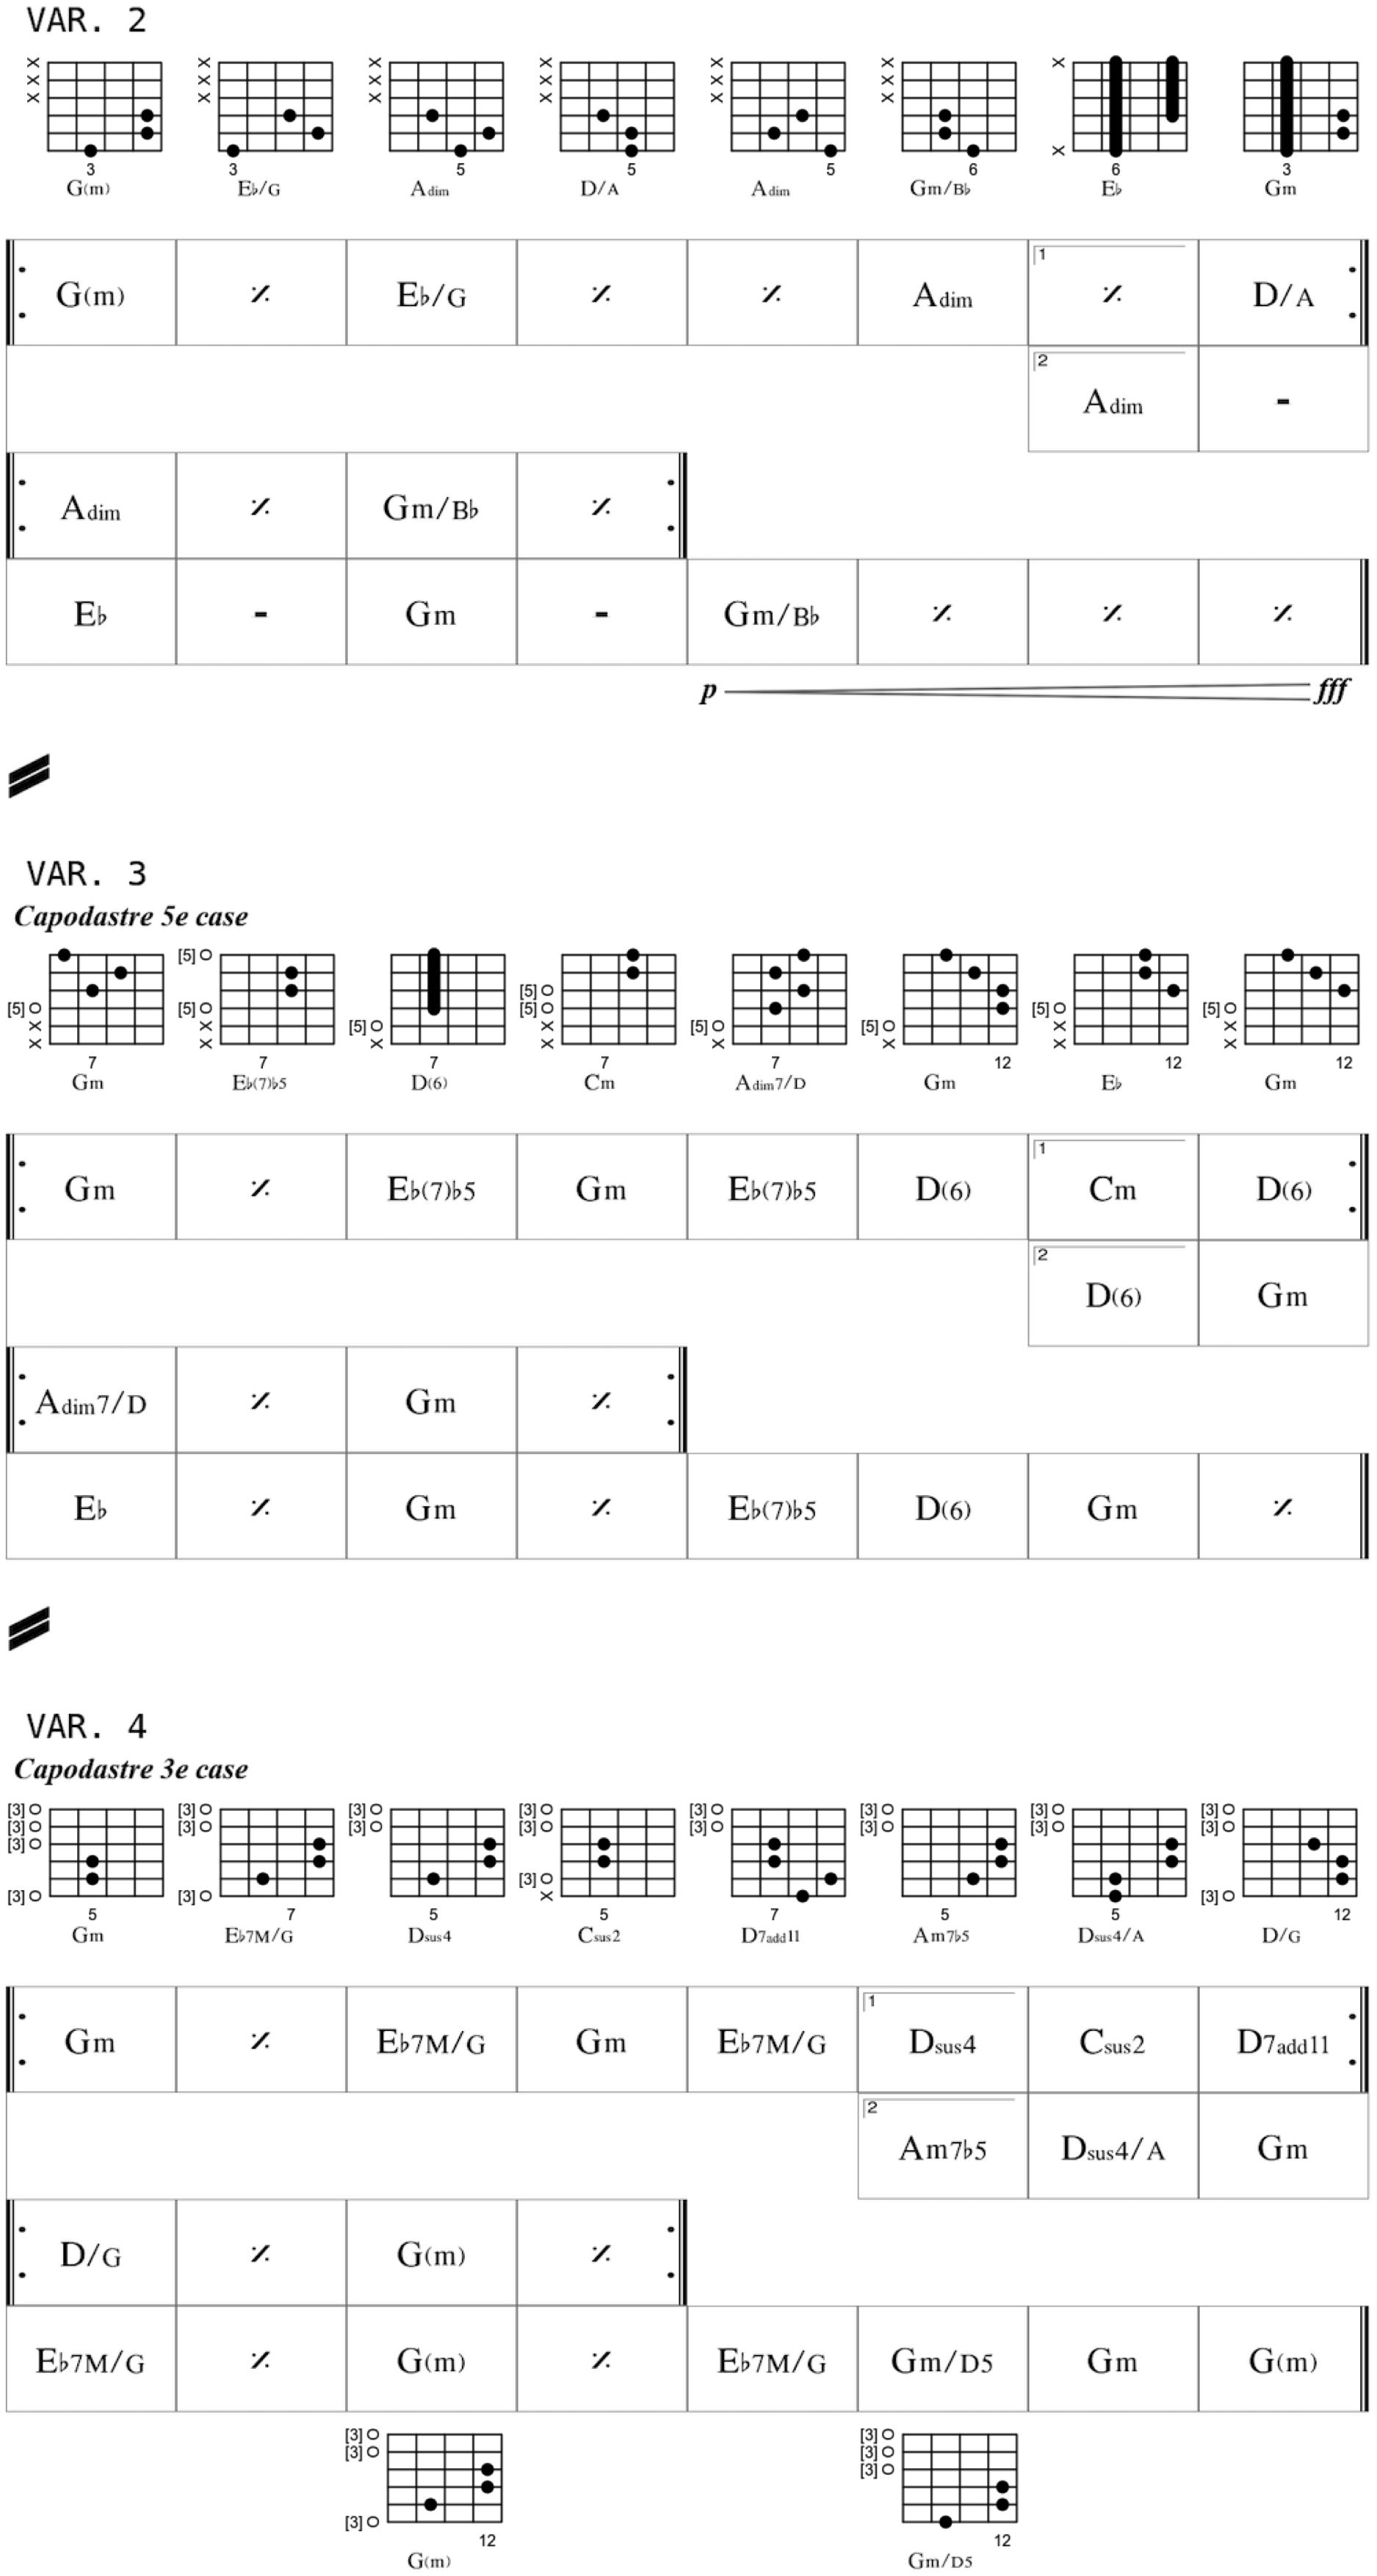
\includegraphics[width=\textwidth]{img/dlc3}
\end{center}
\end{figure}

 \begin{figure}[H]
\begin{center}
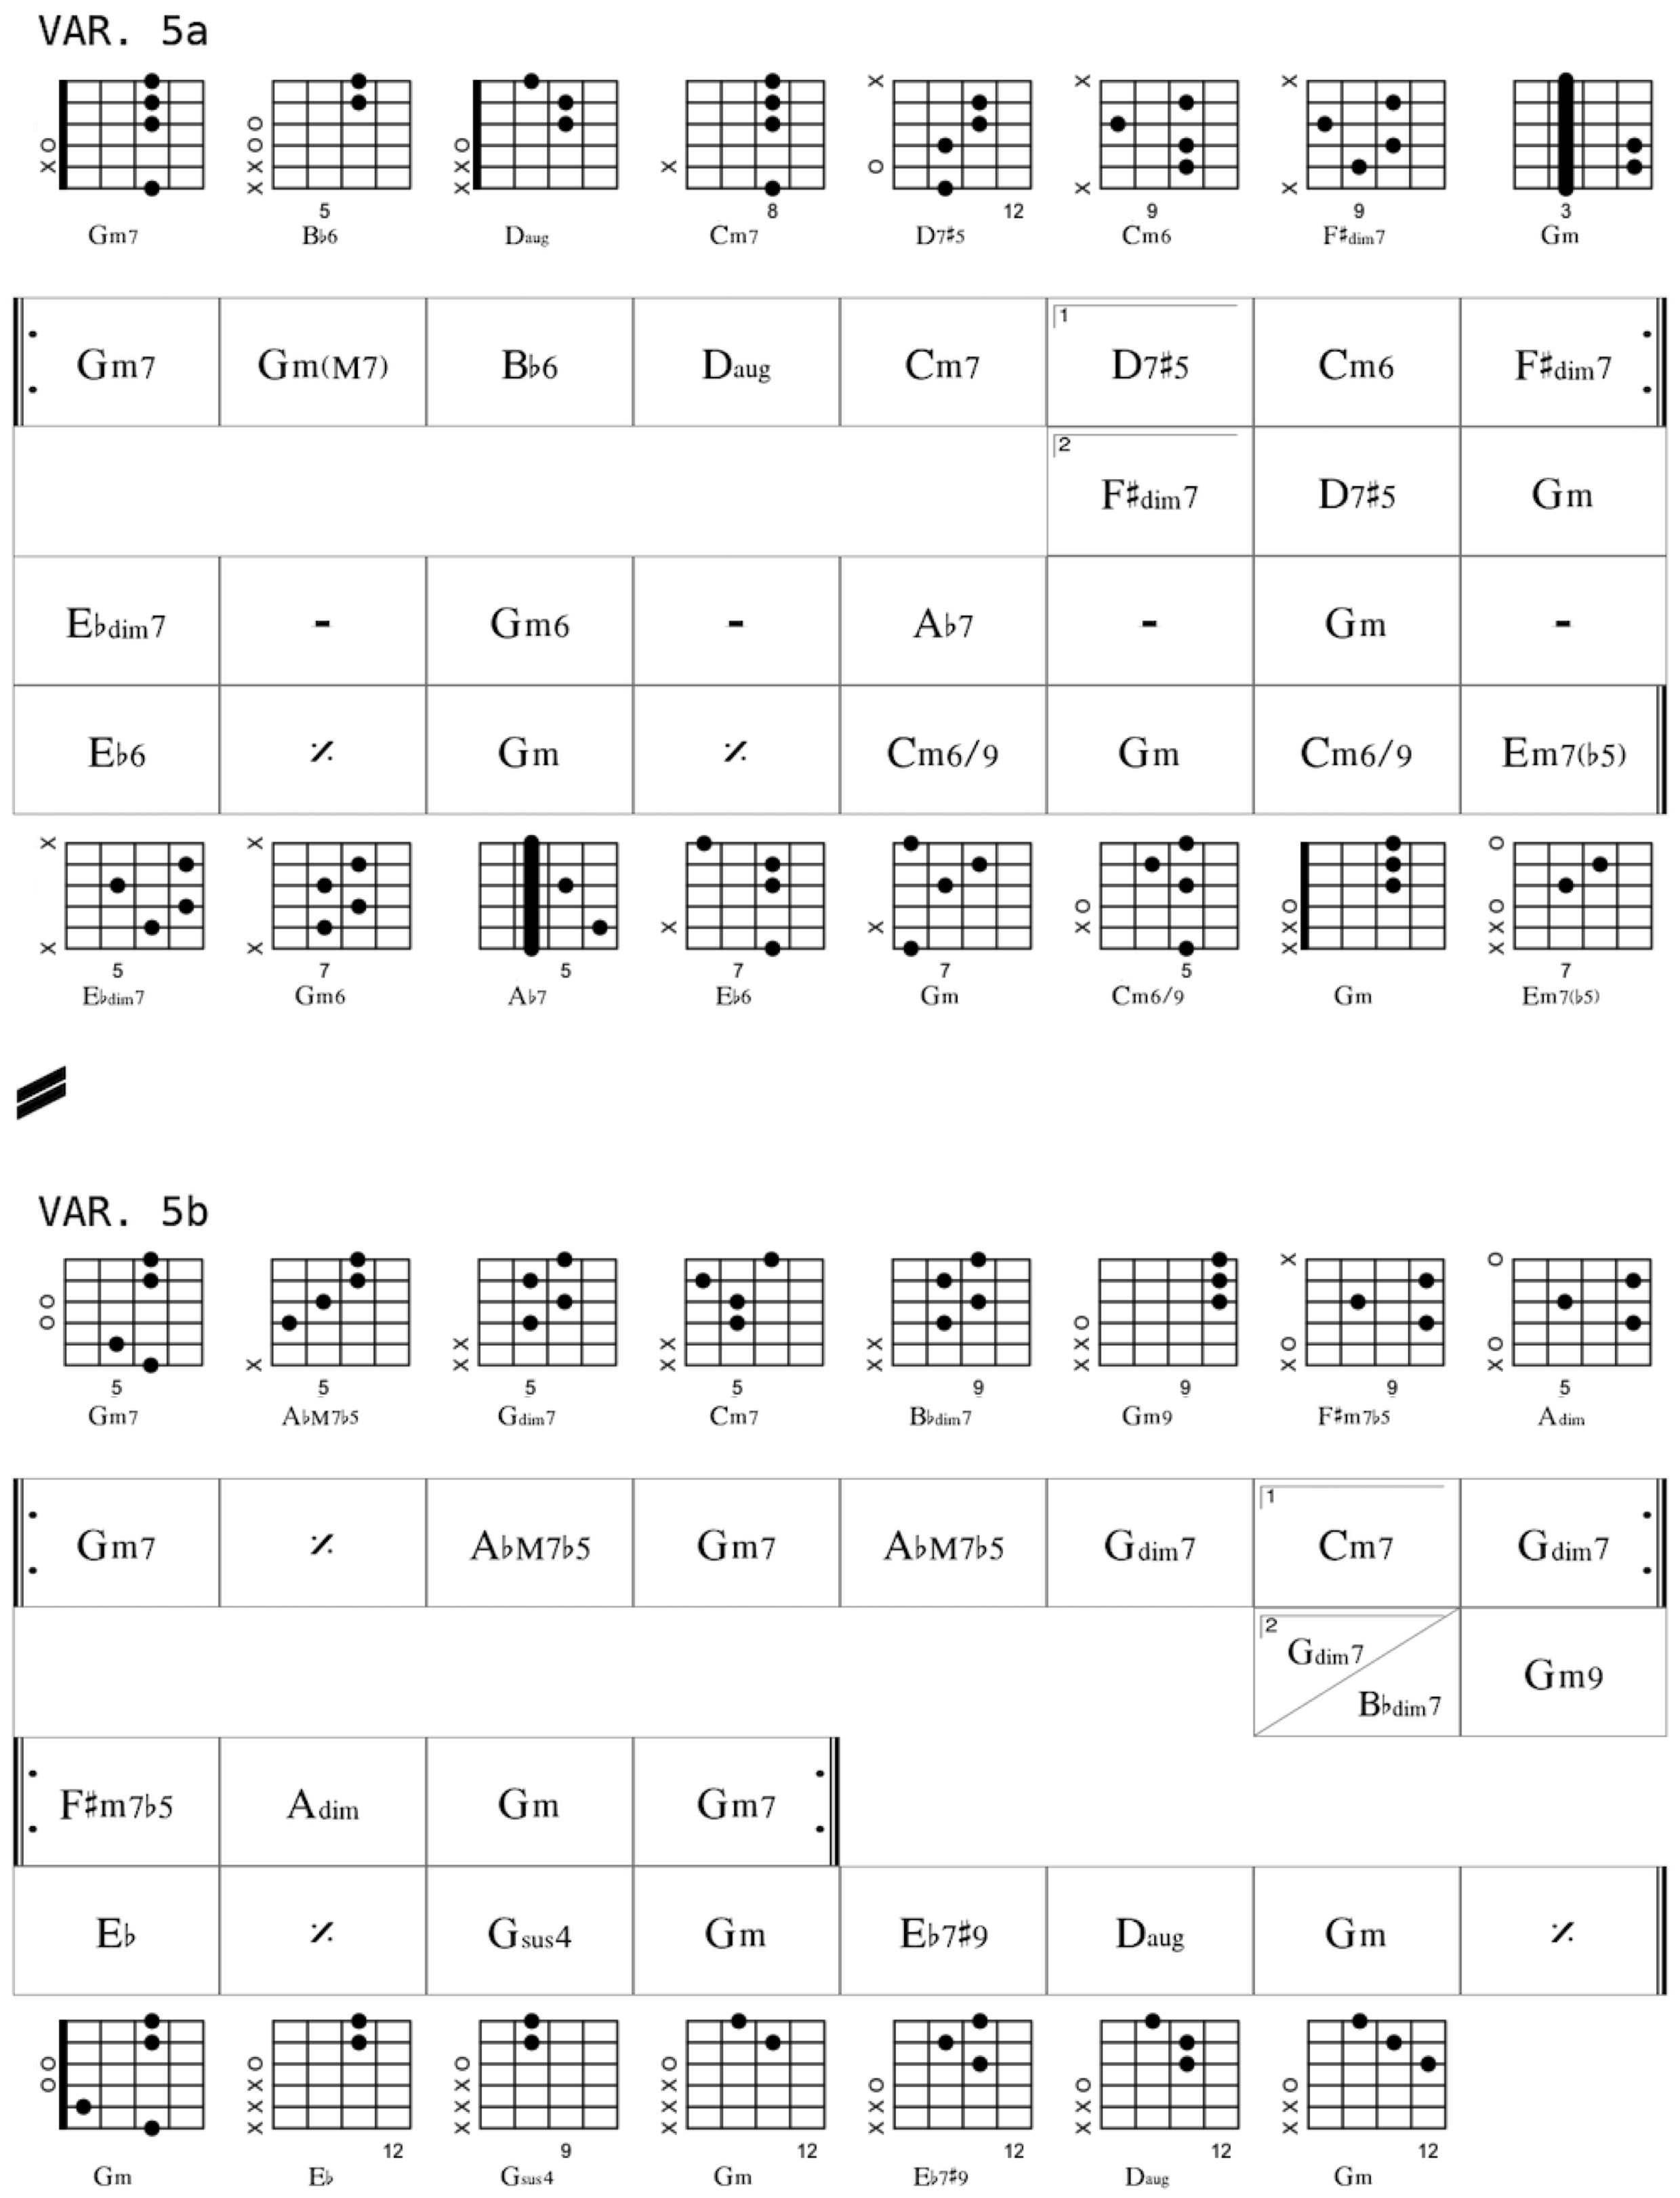
\includegraphics[width=\textwidth]{img/dlc4}
\end{center}
\end{figure}

Voici les combinaisons possibles selon les grilles propos\'{e}es (1 = variation 1, 2 = variation 2, 3 = variation 3 et 4 = variation 4, 5 = variation 5a, et 6 = variation 5b) pour 4 guitaristes: 

1 -- 2 -- 3 -- 4 -- 5 -- 6 -- 12 -- 13 -- 14 -- 15 -- 16 --  23 -- 24 -- 25 --26 -- 34 -- 35 -- 36 -- 45 -- 46 -- 56 -- 123 -- 124 -- 134 -- 135 -- 136 -- 234 -- 235 -- 236 -- 345 -- 346 -- 456 -- 1234 -- 1235 -- 1236 --2345 -- 2346 -- 3456 %-- 12345 -- 12346 -- 23456 -- 123456
 
\bigskip

\subsection*{Th\`{e}me Rythmique -- djemb\'{e}/dum-dum}

Les percussions sont d\'{e}finies ici -- par d\'{e}faut -- par le couple djemb\'{e}/dumdum, mais peuvent bien entendu \^{e}tre adapt\'{e}es selon un \textit{instrumentarium} libre et selon des motifs rythmiques autres, mais apparent\'{e}s.

 %La s\'{e}quence pr\'{e}sent\'{e}e ici est un exemple.
 
 \begin{figure}[H]
\begin{center}
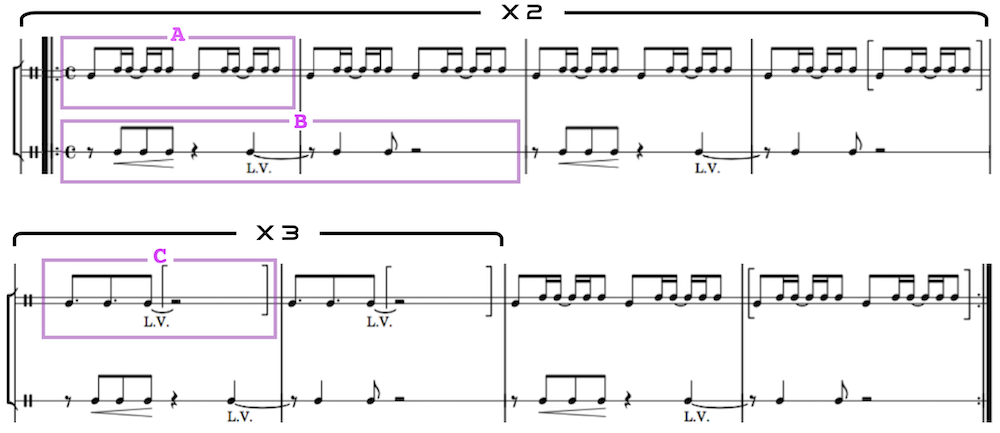
\includegraphics[scale=0.68]{img/dlc5}
\end{center}
\end{figure}

\`{a} l'instar des briques d'une construction, chaque motif rythmique --  ici encadr\'{e} et d\'{e}nomm\'{e} A, B et C -- est agenc\'{e} afin d'entrer dans l'\'{e}laboration d'une s\'{e}quence enti\`{e}re, soit 16 mesures.

Les parties entre crochets doivent \^{e}tre interpr\'{e}t\'{e}es en termes d'articulation et/ou de cadence selon le contexte.
